\documentclass[../report]{subfiles}
\setcounter{section}{0}
\begin{document}

本章では,システム案出しのプロセスについて説明する.
\bunseki{山根春貴}

\section{システム案出し}
知識習得の際に得た知識からグループメンバーそれぞれが認知症に関する別々の分野の問題に着目してシステム案を考えた.
その結果, 1.排泄通知システム, 2.MyGO!, 3.介護者SNS, 4.認知症患者の見守りとプライバシーの両立,5.暴力・暴言行動記録システムの5案が出た.
アイデアの概要を以下で紹介する.
\bunseki{山根春貴}

\subsection{排泄通知システム}
家庭内の介護者(特に家族)を対象とし,認知症の方の排泄時間を事前に通知するシステム.

排泄を行った時間を日々記録し,排泄予測時間前に通知をする.
その記録データが増えるほどより精密な時間に通知してくれるようになる.
記録は便座に圧力センサを導入し,座ったときにセンサが反応,デバイスに自動で記録してくれる.
通知はPepperが音声で行う.
\bunseki{山根春貴}

\subsection{MyGo!}
軽度認知障害者を対象とした散歩支援システム.

モチベーションを向上させるには,手間を減らす必要がある.
手軽に撮れるライフログカメラを使用する.
また歩数計を用いることで使用者が意識せずとも使える.

ウォーキングマップの情報を基に散歩支援システムを提案.
例えば,五稜郭公園に入った時に見どころを音声で知らせる.
クイズを出してクイズに成功するとスタンプなどの報酬を得られる.
\bunseki{山根春貴}

\subsection{介護者SNS}
認知症患者の介護者を対象とした介護者同士での意見交換できる場をつくるシステム.

認知症患者の介護者(家族,ヘルパー),そして地域の認知症サポーターが参加するSNS.
介護者の悩み相談,認知症に関する知識共有ができる.
認知症患者の情報をあらかじめ非公開で登録しておき,行方不明時に周囲数km内の他のユーザーに通知される.
\bunseki{山根春貴}

\subsection{認知症患者の見守りとプライバシの両立}
グループホームのケアスタッフを対象としてカメラを利用した見守りシステムにおけるプライバシ問題の解決と介護者の負担の更なる軽減を目指すシステム.

カメラを用いた見守りシステムは,介護の現場における人手不足問題とさり気ない介護・観察の実現に効果が期待されるが,同時にプライバシ問題も抱えている.
それを解決すべくICタグや画像分析等を利用することで特に注意が必要な場所や場面の映像を選択的に介護者に提供する.
\bunseki{山根春貴}

\subsection{暴力・暴言行動記録}
家庭内の家族(特に家族)を対象とし介護者が認知症患者から受ける暴力・暴言を記録し,傾向や対処法を提示する.

暴言・暴力が実際に起こった際に,アプリを利用して記録してもらう.
詳細細かに記録してもらうのではなく,いくつかの設問に選択式で答えてもらう.
選択項目を分析し介護者側に認知症患者への接し方についてアドバイスを画面に表示させる.
また,回答した設問をグラフ化し,怒りの傾向を可視化できる.
\bunseki{山根春貴}


\section{システム案レビュー}
\subsection{指導教員からのレビュー}
2017年5月26日,指導教員からシステム案出しで出たシステム案のレビューを頂いた.
頂いたレビューの一部を以下に紹介する.
\begin{enumerate}
    \item 排泄通知システム
        \begin{itemize}
            \item 排泄感知装置をつけるのは嫌がりそう.
            \item 記録をするときデータの入力はどうするの?
        \end{itemize}
    \item MyGo!
        \begin{itemize}
            \item 大枠としては良い.自由に散歩できることは認知症患者にこんな良い点がある,というアピールが必要である.自由に徘徊できる街,という事例がある\cite{haikai}.
            \item 症状に合わせたシステムの提案である必要がある.
        \end{itemize}
    \item 介護者SNS
        \begin{itemize}
            \item 既存のアプリとの違い,利点等を説明に入れると良いかも.
            \item 函館市の話では,徘徊者を見つけたらすぐに警察に報告することになっている.
        \end{itemize}
    \item 認知症患者の見守りとプライバシーの両立
        \begin{itemize}
            \item プライバシーの危機を感じているのは患者か?対象者は?
            \item 介護者が働きにくいと思う環境から,介護者をハッピーにするシステムへ.
        \end{itemize}
    \item 暴力・暴言行動記録システム
        \begin{itemize}
            \item 最終的な目的は暴力・暴言を減らすことなのか,暴言暴力に強くなることなのか?
            \item 暴力・暴言に対してのノウハウを家族に伝えるために,記録して蓄積・統計を取るというのはどれくらい効果があるのか.
        \end{itemize}
\end{enumerate}
\bunseki{山根春貴}

\subsection{函館認知症の人を支える会の代表者からのレビュー}
2017年5月31日,公立はこだて未来大学で行われた認知症サポーター養成講座を受講した.
この講座では,認知症患者との接し方など知識習得,自分たちで考えたシステム案に対するレビューを目的として受講した.
講師の方から頂いたレビューの一部を以下に紹介する.
\begin{enumerate}
    \item 排泄通知システム
        \begin{itemize}
            \item 食事水分のとり方によって変わる.
            \item 年寄りは回数が増える.しかし介護者のストレスを軽減する良いアプローチ.
        \end{itemize}
    \item MyGo!
        \begin{itemize}
            \item 最初のきっかけを与えるということを考えて欲しい.
            \item 万歩計の歩数に応じて何か還元できるものがあれば対象者も積極的にやってくれるようになるのでは?
        \end{itemize}
    \item 介護者SNS
        \begin{itemize}
            \item この考え方はすでにある.地域の助け合いネットワークとしては効果がある.地域ネットワークの中で,協力し合うとかだと発見に近くなる.
            \item こういう考え方は普段は写真を使わない.だから使うとなると効果は出ると思う.でも本人や家族の了解なしでやるのはどうだろうか.
        \end{itemize}
    \item 認知症患者の見守りとプライバシーの両立
        \begin{itemize}
            \item 実際にカメラが入っているグループホームがある?認知症患者側が嫌だという論文はなくて,介護している側が嫌だという論文があった?
            \item 見守りとプライバシーは相反すること.徘徊を防ぐのであれば出口ぜんぶ閉じる.出ていった後は難しい.どういうところを見守るかを明確にしないと考えまとまらないのでは.
        \end{itemize}
    \item 暴力・暴言行動記録システム
        \begin{itemize}
            \item パターン化出来ない.問題は接し方.それをグラフ化,何か作るというのはなかなか難しい.フィードバックもいつも同じものではない.家族の人間関係にもよる.一番はその人が安心できる,というもの.この人の前だと何言っても良いんだ,と思える人.暴言暴力が起こるというのは,接し方が原因.一番難しい分野.
        \end{itemize}
\end{enumerate}
\bunseki{山根春貴}

\subsection{京都府立医科大学成本医師からのレビュー}
2017年6月7日,京都府立医科大学の成本迅医師とSkypeによる会議を行った.
この会議では,システム案に対してのコメントを頂いたり,成本迅医師の要望を聞いたりした.
会議で成本迅医師から頂いた意見の一部を以下に紹介する.
\begin{enumerate}
    \item 排泄通知システム
        \begin{itemize}
            \item 健常者は日中にトイレに行き,夜は寝てるだけ.老いてくると夜もトイレに.こういった排泄のリズムを録ることが出来れば良い(高齢化に伴う排泄のリズムの変化を見つける).生活の中にどれだけ自然な形でインストールするか,というのが重要.
        \end{itemize}
    \item MyGo!
        \begin{itemize}
            \item 函館のウォーキングマップに沿った形で良い.ロボホンを首からかけて移動するとクイズを出したり,案内したり,というのは少し似ている.これはスマホをぬいぐるみに入れるというのでも代用できる.高齢者の方と一緒に歩いて,あとで振り返れると良い.
        \end{itemize}
    \item 介護者SNS
        \begin{itemize}
            \item 介護者特有の悩みを共有するできる場にする.
            \item 行方不明の通知は先行研究などで色々やられていて,いざというときだけ公開するのは良い.
        \end{itemize}
    \item 認知症患者の見守りとプライバシーの両立
        \begin{itemize}
            \item ケアの負担軽減,というのは日本でかなり必要とされている技術.様々なものが作られているが,全然導入されていない.というのも機械アレルギーがある.現状で満足してしまっている.
        \end{itemize}
    \item 暴力・暴言行動記録システム
        \begin{itemize}
            \item 暴言暴力も施設入居のきっかけ.行動療法は患者の行動を見て,療法を提示するが,今はアナログ.これをアプリ化すればより便利になるのでは.
            \item やはり可視化するというのは非常に重要.記録することで,自覚しているしんどさと実際に起きていることが違ったりする.記録するだけで問題が解決することもある.いかに簡単に記録してもらうか.
        \end{itemize}
\end{enumerate}
\bunseki{山根春貴}

\subsection{もの忘れカフェでのレビュー}
2017年6月17日,函館総合福祉センターで行われたもの忘れカフェに参加した.
このイベントでは,施設のことや認知症患者に詳しい方にシステム案を提案し,レビューを頂いた.
時間の都合上,「排泄通知システム」と「MyGO!」の2案だけ提案した.もの忘れカフェで頂いたレビューの一部を以下に紹介する.
\begin{enumerate}
    \item 排泄通知システム
        \begin{itemize}
            \item 排泄や食事などの記録をとる期間は相当かかるのではないか?
            \item トイレに行った記憶がなくなって,トイレに行きたいという人もいる.
        \end{itemize}
    \item MyGo!
        \begin{itemize}
            \item ロボットを使うことについて,認知症患者の方がしゃべる→録音→すぐ再生する,というシステムがあった.最初は重度の認知症患者の方でも興味を示していたが,そのうち全く興味を示さないようになった例がある.
        \end{itemize}
\end{enumerate}
\bunseki{山根春貴}


\section{システム案の再検討}
\subsection{新しいシステム案}
頂いたレビューや知識習得からシステム案の改善を繰り返してきた.
しかし,どのシステム案もいくつか問題点が残るものとなり,アイデアの試行錯誤が続いた.
そこで,今までの案から建設的なアイデアが生まれることを期待して,案の再考という流れに至った.
再考するまでのシステム案は,認知症患者やその介護者に関する問題を解決するシステム案を考えていた.
再考する際,認知症になる前段階の高齢者を対象とし,システム案を考えた.
システム案を考え,グループで出た方向性を以下にまとめた.
\begin{itemize}
    \item 認知症ではない高齢者の認知症のリスクを減らす
    \item ライフログデータを活用したコミュニケーションや生活習慣の見直しの切っ掛け作りをする
\end{itemize}
この方向性を整理してまとまった案が「認知症予防のための食習慣改善システム」である.
運動や睡眠といった生活習慣の中で食習慣に着目した理由は,植木(2005)の調査から健常者と比較して,アルツハイマー型認知症患者の食生活バランスが崩れていることが明らかになっている\cite{ueki}からである.
システムのイメージ図を以下\ref{fig:sys-image}に示す.
\begin{figure}[htbp]
    \begin{center}
        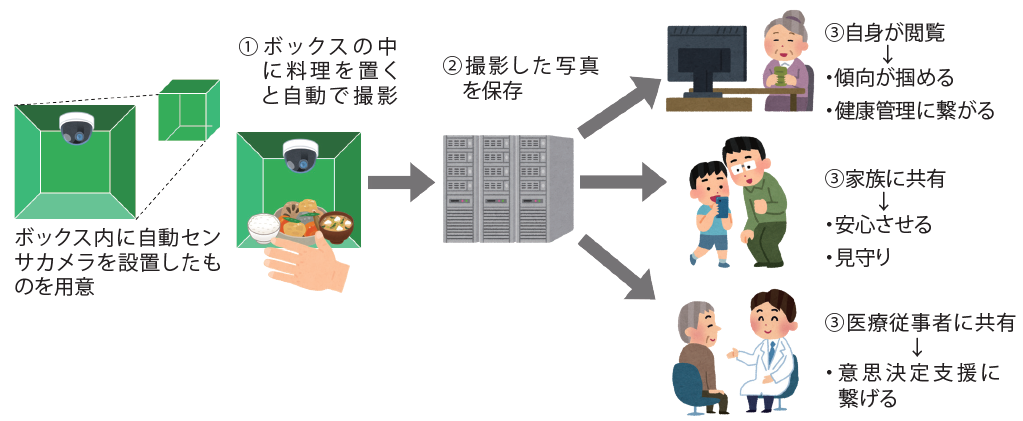
\includegraphics[width=10cm]{imgs/system-overview.png}
        \caption{システムのイメージ図}
        \label{fig:sys-image}
    \end{center}
\end{figure}
\bunseki{山根春貴}

\subsection{新しいシステム案に対するレビュー}
プロジェクト学習中に行われたレビュー会や中間発表会で「認知症予防のための食習慣改善システム」に対するレビューを頂いた.
「意思決定支援につながった例はあるのか」といった先行研究についての質問や高齢者自身の閲覧のデータの見せ方,料理の撮影方法について多くのレビューを頂いた.
\bunseki{山根春貴}

\end{document}
